\documentclass{standalone}
\usepackage{preset}
\begin{document}
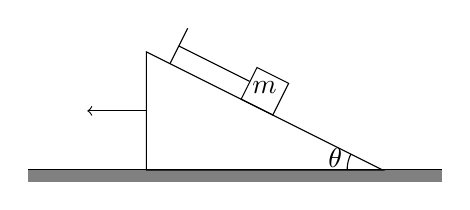
\begin{tikzpicture}[x=15mm,y=15mm]
	\draw(-1,0)--(2.5,0);
	\draw[draw=none,fill=gray](-1,0)rectangle(2.5,-.1);
	\draw(0,0)--(2,0)--(0,1)--cycle;
	\draw(1.7,0)arc(180:153.43:.3);
	\draw[->](0,.5)--+(-.5,0);
	\draw(.2,.9)--+(.15,.3);
	\draw(.275,1.05)--+(.6,-.3);
	\draw[rotate=-26.57](.45,.895)rectangle+(.3,.3);
	\draw(1,.7)node{$m$};
	\draw(1.6,.1)node{$\theta$};
\end{tikzpicture}
\end{document}
